\subsection{Fragen und Antworten zum Text von \textcite{rabinowitz_section_2013}}
\subsubsection{Was charakterisiert nach \textcite{rabinowitz_section_2013} einen partizipativen Zugang zur Planung einer Community Intervention?}
Ein Ansatz, bei dem jeder, der von der Intervention betroffen ist, eine Stimme bei der Planung hat. Dazu geh"oren \emph{Mitglieder der Organisation} die die Ma"snahme durchf"uhrt, \emph{Mitglieder der Zielpopulation}, \emph{Offizielle}, \emph{interessierte B"urger}, etc.

Diese Personengruppen k"onnen entweder pers"olich beteiligt sein, oder aber durch einen Interessensvertreter repr"asentiert werden.

\subsubsection{Was muss in Bezug auf Angeh"orige von Gruppen, die einen niedrigen Status haben, beachtet werden?}
Es kann sein, dass sie besondere Unterst"utzung brauchen. Zum einen, um zu \emph{lernen}, wie das Programm funktioniert. Zum anderen, um auch tats"achlich zu \emph{glauben}, dass ihre Meinung wertgesch"atzt und beachtet wird.

\subsubsection{Was sind m"ogliche Vorteile eines partizipativen Zugangs? Was sind m"ogliche Nachteile?}
\begin{itemize}
        \item \textbf{Vorteile:}
                \begin{itemize}
                        \item \emph{sense of ownership}
                        \item bessere Glaubw"urdigkeit in der Community
                        \item mehr und unterschiedliche Ideen und Sichtweisen
                        \item Realit"aten der Community werden ber"ucksichtigt (z.B. Ramadan)
                        \item wichtige \emph{player} involviert
                        \item oft ausgeschlossene Gruppen werden geh"ort
                        \item Vermittlung von F"ahigkeiten, die auch "uber die Intervention hinaus Bestand haben
                        \item Etablierung von Beziehungen zwischen Community Mitgliedern
                        \item Bildung von Vertrauen (zwischen Organisation und Community, aber auch unter Community Mitgliedern)
                        \item in Einklang mit den Idealen von \emph{grass roots}- und Non-Profit Organisationen
                        \item Respekt f"ur jeden in der Community
                        \item sollte aus Gr"unden der Logik (?) wirksam sein
                        \item Dinge werden so gemacht, wie es sein soll
                \end{itemize}
        \item \textbf{Nachteile:}
                \begin{itemize}
                        \item braucht mehr Zeit
                        \item Mitglieder der Zielpopulation und Experten k"onnen nicht "ubereinstimmen
                        \item k"onnte sehr viel Lernen erfordern (auf Seiten der Organisation und der Mitlgieder)
                        \item ein Einzelner kann den Prozess torpedieren
                        \item schwer, alle an einen Tisch zu bekommen
                        \item erfordert Geduld und Commitment von allen Beteiligten
                \end{itemize}
\end{itemize}

\subsubsection{Was sind die vier Stufen der Partizipation? Wann sind sie jeweils angemessen?}
Hmm\ldots eigentlich sind es f"unf Stufen. Im folgenden die Einzelheiten.\\

\emph{Information} ist angemessen, wenn die Ma"snahme bereits beschlossen ist (z.B. von einem Sponsor), man nur "uber eine bereits bestehende Ma"snahme berichtet, oder die Mitglieder f"ur eine eventuelle sp"atere Ma"snahme informiert.

\emph{Konsultation} ist angemessen, wenn eine bereits bestehende Ma"snahme evaluiert oder verbessert werden soll, es eine Reihe von Vorschl"agen gibt, aus denen ausgew"ahlt werden soll, oder wenn aus technischen Gr"unden nur bestimmte Gruppen ber"ucksichtigt werden k"onnen.

\emph{Zusammen entscheiden} ist angemessen, wenn \emph{ownership} gef"ordert werden soll, man frische Ideen braucht, man Leute einbeziehen kann, die direkt betroffen sind, es Commitment gibt, die Leute zu unterst"utzen, die es n"otig haben, und wenn genug Zeit da ist.

\emph{Zusammen handeln} ist angemessen, wenn die Intervention so effektiver ist (als wenn man sie alleine durchf"uhrt), die Sponsoren es verlangen, es ein Commitment zur Entwicklung einer echten Partnerschaft gibt, jeder von der gemeinsamen Handlung profitiert, oder das Ziel der Intervention darin besteht, die Betroffenen in die Lage zu versetzen, die Intervention alleine weiterzuf"uhren. 

\emph{Lokale Initiativen zu unterst"utzen} ist angemessen, wenn es ein Commitment zu \emph{empowerment} gibt, die Community den Wunsch und wenigstens einige Tools hat, die man braucht, Training bereitgestellt werden kann, oder wenn die Organisation nur begrenzte Ressourcen oder Ziet zur Verf"ugung hat.

\subsubsection{Was muss beachtet werden, wenn Konsultationen durchgef"uhrt werden?}
Es bringt nichts, die Leute nach ihrer Meinung zu fragen und diese dann zu ignorieren. Das ist sogar schlimmer, als gar nicht zu fragen.

\subsubsection{In welchen Situationen ist Partizipation nicht angemessen? Nennen Sie ein Beispiel f"ur eine solche Situation!}
\begin{itemize}
        \item keine Zeit
        \item Community Mitglieder zu stark abgeschottet
        \item keine M"oglichkeit zur notwendigen Unterst"utzung
        \item Zielpopulation nicht interessiert an Ma"snahmen
        \item technisches Wissen notwendig, dass niemand hat
        \item logistische Probleme (z.B. Distanz)
        \item kein Vertrauen zwischen Organisation und Mitgliedern
\end{itemize}

\subsubsection{Wer sollte in einen partizipativen Prozess involviert werden?}
Siehe Fig. \ref{fig:rabinowitz1}.

\begin{figure}[hb!]
        \begin{center}
                \begin{tikzpicture}[mindmap,font=\large\scshape,grow cyclic,every node/.style={concept, execute at begin node=\hskip0pt},concept color=black!20,
                        level 1/.append style={level distance=4cm,sibling distance=1cm,sibling angle=90, font=\scshape}]
                        \node{Wer sollte involviert werden?}
                        child{node{Targets}}
                        child{node{Agents}}
                        child{node{Interessierte B"urger}}
                        child{node{Organisationsmitglieder}};
                \end{tikzpicture}
        \end{center}
        \caption{Personengruppen, die an einer partizipativen Ma"snahme teilnehmen sollten (nach \textcite{rabinowitz_section_2013}).}
        \label{fig:rabinowitz1}
\end{figure}

\subsubsection{Was sind die Schritte, die laut Rabinowitz f"ur einen partizipativen Planungsprozess durchgef"uhrt werden m"ussen?}
Die drei Schritte sind \emph{Stakeholder rekrutieren}, \emph{den Planungspozess zusammenzubringen} (engl.: convene) und \emph{den Planungsprozess aufrecht zu erhalten}. Sie dazu auch Fig. \ref{fig:rabinowitz2}.
\begin{figure}[hb!]
        \begin{center}
                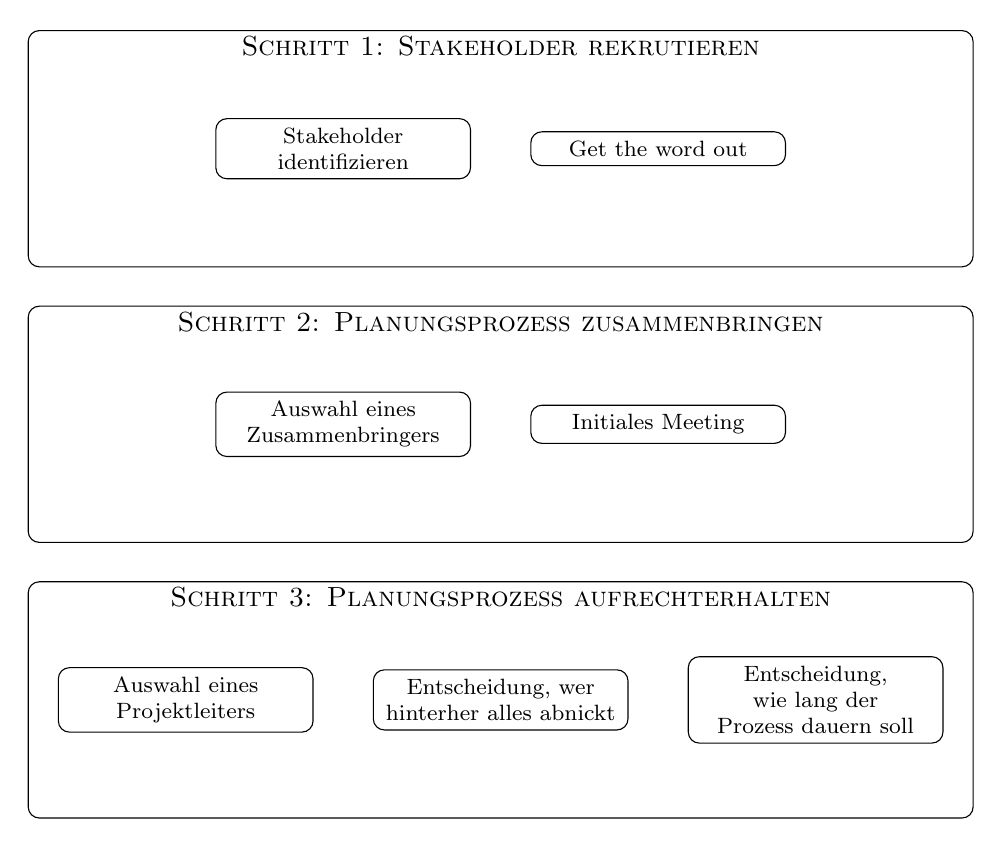
\begin{tikzpicture}[level1/.style={rounded corners},
                        level2/.style={shape=rectangle,draw,rounded corners,text centered,font=\footnotesize, text width=3cm}
                        ]
                        %Schritt 1: Stakeholder rekrutieren
                        \node at (0,2.8) {\scshape Schritt 1: Stakeholder rekrutieren};
                        \draw [level1] (-6,0) rectangle (+6,3);
                        \node [level2] at (-2,1.5) {Stakeholder identifizieren};
                        \node [level2] at (+2,1.5) {Get the word out};
                        %Schritt 2: Planungsprozess zusammenbringen
                        \node at (0,-0.7) {\scshape Schritt 2: Planungsprozess zusammenbringen};
                        \draw [level1] (-6,-3.5) rectangle (+6,-0.5);
                        \node [level2] at (-2,-2) {Auswahl eines Zusammenbringers};
                        \node [level2] at (+2,-2) {Initiales Meeting};
                        %Schritt 3: Panungsprozess aufrecht erhalten
                        \node at (0,-4.2) {\scshape Schritt 3: Planungsprozess aufrechterhalten};
                        \draw [level1] (-6,-7) rectangle (+6,-4);
                        \node [level2] at (-4,-5.5) {Auswahl eines Projektleiters};
                        \node [level2] at (-0,-5.5) {Entscheidung, wer hinterher alles abnickt};
                        \node [level2] at (+4,-5.5) {Entscheidung, wie lang der Prozess dauern soll};
                \end{tikzpicture}
        \end{center}
        \caption{Schritte und Unterschritte f"ur den partizipativen Planungsprozess nach \textcite{rabinowitz_section_2013}.}
        \label{fig:rabinowitz2}
\end{figure}

\subsubsection{Sollten m"oglichst immer alle Beteiligte zu Treffen eingeladen werden? Begr"unden Sie Ihre Antwort!}
Ein gro"ses Meeting k"onnte einsch"uchternd wirken und manche davon abhalten, etwas zu sagen oder "uberhaupt erst zu kommen.

